%%%%%%%%%%%%%%%%%%%%%%%%%%%%%%%%%%%%%%%%%%%%%%%%%%%%%%%%%%%%%%%%%%%%%%%%%%%%%%%%
% 								FRAME OF THE THESIS 						   %
%%%%%%%%%%%%%%%%%%%%%%%%%%%%%%%%%%%%%%%%%%%%%%%%%%%%%%%%%%%%%%%%%%%%%%%%%%%%%%%%
\subsection{A World Full of Embedded Cryptography}
\label{sec:world_crypto}

Research in \gls{cryptology} has always benefited the competition between its two sides, namely \gls{cryptography} and \gls{cryptanalysis}.
Depending on the epochs, one of the two sides may have taken the advantage on the other.
Some important events in History, such as wars and conflicts, have been indirectly impacted by this latent rivalry~\cite{singh_code_book_1999}.
Yet, the past forty years have seen the emergence of a period in which \gls{cryptography} has taken the advantage.
Along with other external factors, this has implied a pervasiveness of \gls{cryptography}, shaping our mordern lives.
This trend may be explained by three factors that we detail hereafter:
\begin{enumerate}
	\item The emergence of \emph{trust} in \gls{cryptography}.
	\item The digitization of our modern world.
	\item The advent of standardization in cryptographic protocols.
\end{enumerate}


\paragraph{The Emergence of Trusted Primitives.}
Crypto-systems may be seen as the set of \glspl{primitive} which, combined to each other, provide the security functionalities required by the user, such as confidentiality, integrity, authenticity, non-repudiation.
As such, the security and reliability of the whole crypto-system is grounded on those of the primitives.
The quest of perfect primitives is so far a mission that motivates most of the research work in \gls{cryptology}.

% Emergence of secure primitives
Hopefully, over the last decades, the \gls{cryptology} community has seen the emergence of \emph{secure} primitives, which currently allows to bring enough trust in the crypto-systems.
The notion of security of such primitives may be defined in two ways, that we recall hereafter.
\begin{itemize}
	\item \textbf{Provably secure}: A primitive is said to be \emph{provably secure} \gls{iff} defeating this primitive is strictly equivalent to solving a known mathematical problem, so that any attacker willing to defeat the primitive would have to solve this mathematical problem.
	If the latter is known to be intractable enough, then this brings strong guarantees in the security of the primitive.
	As examples, the Diffie-Hellman key exchange protocol relies on the \emph{discrete logarithm} problem~\cite{diffie_new_1976}, while the \gls{rsa} protocol used in \gls{asym_crypto} relies either on the factorization of large prime numbers~\cite{rsa_1978} or on the so-called \gls{rsa} problem~\cite{boneh_breaking_1998}.
	Both problems are known to be intractable on classical computers.
	\item \textbf{Reputed secure}: A primitive is said to be \emph{reputed secure} \gls{iff} no efficient attack has been emphasized over a long period.
	Although this does not rigorously prove the security of the primitive, the fact that many people from the research community in \gls{cryptology} have attempted to find a vulnerability without success gives strong evidences of the soundness of the given primitive.
	This is particularly the case of the \gls{aes}, that we will further describe in \autoref{sec:intro_aes}: the best known attack requires a complexity that is roughly of the same order of magnitude as a brute-force attack enumerating the \(2^{128}\) possible keys, which makes a practical attack intractable~\cite{bogdanov_biclique_2011}.
\end{itemize}

Although the security property of the mentioned primitives may vary in the next years, in the case where new attack paths might be found,%
\footnote{Actually quantum computers would be able to efficiently resolve prime factorization and discrete logarithm~\cite{shor_poly_1994}.
Hopefully, quantum computers are not up to date yet, which would let enough time to find \emph{post-quantum} algorithms resilient to such threat.
The \gls{nist} is currently running a competition to select new post-quantum designs.
The interested reader may refer to \url{https://csrc.nist.gov/projects/post-quantum-cryptography}.}
it is noticeable that the mentioned primitives have earned their reputation over a quite long period of time, thereby reinforcing trust in them.

\paragraph{From (Electro)-Mechanical to Electronic Systems.}
Crypto-systems propose solutions to secure communications asking some secret keys for computations on which is ground their security.
Keys are represented as long strings from an alphabet specified by the underlying \glspl{primitive}.
A sound crypto-system must let the parties communicating with each other to be able to securely store and manipulate those keys, without delivering them in clear over insecure channels.
However, from a practical perspective, using trusted \glspl{primitive} is not enough to spread their use: they must be efficiently usable in any context.
Thanks to the progressive replacement during the 20-th century of crypto-systems implemented on mechanical or electro-mechanical devices, by fully electronic devices realizing such operations is nowadays drastically faster~\cite{singh_code_book_1999}. 

% Intro smart cards
As an example, \emph{smart cards} were historically conceived as a practical solution to such a key storage issue: they consist in small devices that a user can easily carry around with, which not only store secret keys as long strings of bits, but also are able to internally perform cryptographic operations, in such a way that they can be involved in secure communication protocols, that do not require the delivering of secret keys.
Smart cards are pocket-sized plastic-made cards equipped with a secure component, which is typically an integrated circuit containing some computational units and some memories.
They have been patented by Moreno in 1974~\cite{moreno_methods_1974} -- as a memory device -- and Ugon in 1977~\cite{ugon_portable_1977} -- a a computing device.

Today, about 40 years after its invention, smart cards still have a huge diffusion, both in terms of applicative domains and in terms of quantity of copies.
Indeed, they serve as credit or ATM cards, healthy cards, ID cards, public transportation payment cards, fuel cards, identification and access badges, authorization cards for pay television, \etc{}
Slightly changing the card support, we find other applications of the same kind of integrated circuits, for example the mobile phone \glspl{sim} and the electronic passports.
In terms of quantity, a marketing research found out that in 2014, 8.8 billion smart cards have been sold~\cite{ABI}, \ie{}, the same order of magnitude of the global population.

In addition to smart cards, the recent growing and variation of security needs lead to the development and specification of other kinds of secure solutions, for example the \gls{tpm}, which is a secure element providing cryptographic functionalities to a motherboard, or completely different solutions based on software layers, which are today in great expansions.
An example is provided by the \gls{tee}, a software environment of the main processor of a smartphone or tablet, designed to assure resistance to software and even hardware threats.

\paragraph{The Standardization of Cryptographic Primitives.}
The last ingredient contributing to the spread of applications relying on \gls{cryptography} is the standardization of the protocols and the primitives.
Standardization enables to make different crypto-systems compatible, so that any couple of instances (people, device) equipped with a same cryptographic primitive can then securely communicate, without necessarily having to first agree on a communication protocol, since the standardized one is implicitly chosen.
Standardization is usually done by a third part, able to endorse the security of the proposed primitive after comprehensively verifying its security.
Typically, this is done by institutions or government agencies such as the \gls{nist}.
In this thesis, we will mainly focus on a standard edited by the latter institution, called \gls{aes}, presented in \autoref{sec:intro_aes}.
The economic impact of the adoption of this standard, along with the two other factors we previously described, has been evaluated 2018 to 250 billion dollars at a global scale, according to a \gls{nist} report~\cite{nist_eco_impact_2018}.

\subsection{The \glsfirst{aes}}
\label{sec:intro_aes}
In this thesis, we will mainly focus on the \gls{aes} algorithm,%
\footnote{
	This algorithm is also known under the name of \emph{Rijndael} after the name of its two creators Vincent Rijmen and Joan Daemen.
}
though many aspect may be generalized to other algorithms.
The \gls{aes} is a \gls{block_cipher} used for encryption or authentication in embedded devices.
Its specifications are established by the \gls{fips} publication 197 released by the \gls{nist} in 2001~\cite{nist_2001}.
It proceeds blocks of 128 bits by running several \emph{rounds}, as depicted in \autoref{fig:aes_rounds}, composed of elementary operations, called \(\ark, \sub, \sr, \mc\), thanks to a secret key of 128 bits as well.%
\footnote{
	There exists \gls{aes} versions using keys of respectively 192 and 256 bits.
	In this thesis, we will mainly focus on the 128 bit version of the algorithm, without loss of generality.
}
\begin{figure}
	\centering
	\tikzstyle{block} = [rectangle, draw, fill=ceablue!20, text width=8em, text centered, rounded corners, minimum height=2em, node distance = 1cm]
\tikzstyle{decision} = [diamond, draw, aspect=2.5, fill=ceablue!20, text width=4.5em, text badly centered, node distance=1.5cm, inner sep=0pt]
\tikzstyle{line} = [draw, -latex']
\begin{tikzpicture}
    \node[block, fill=ceadarkred!20] (pt) {Plaintext};
    \node[block, fill=ceadarkred!20, left of = pt, node distance = 5cm] (key) {Key};
    \node[block, below of = pt] (ark){\ark{}};

    \node[block, below of = ark] (sb) {\sub{}};
    \node[block, below of = sb] (sr) {\sr{}};
    \node[block, below of = sr] (mc) {\mc{}};
    \node[block, below of = mc] (ark2) {\ark{}};
    \node[block, left of = ark2, node distance = 5cm] (ks) {\ks{}};
    \node[decision, below of = ark2] (nRound) {\(n = N\)?};
    \node[block, below of = nRound, node distance=2cm] (sb2) {\sub{}};
    \node[block, below of = sb2] (sr2) {\sr{}};
    \node[block, below of = sr2] (ark3) {\ark{}};

    \node[block, fill=cealime!20, right of = mc, node distance = 5cm] (npp) {\(n \leftarrow n+1\)};

    \path[line] (pt) -- (ark);
    \path[line] (key) |- (ark);
    \path[line] (nRound) -| node[midway, fill=white]{No} (npp);
    \path[line] (npp) |- (sb);
    \path[line] (ark) -- (sb);
    \path[line] (sb) -- (sr);
    \path[line] (sr) -- (mc);
    \path[line] (mc) -- (ark2);
    \path[line, dashed] (key) -- (ks);
    \path[line] (ks) -- (ark2);
    \path[line] (ark2) -- (nRound);
    \path[line] (nRound) -- node[midway, fill=white] {Yes} (sb2);
    \path[line] (sb2) -- (sr2);
    \path[line] (sr2) -- (ark3);
    \path[line, dashed] (ks) |- (ark3);
    
\end{tikzpicture}
	\caption{The rounds of \gls{aes}.}
	\label{fig:aes_rounds}
\end{figure}
The \gls{diffusion} is ensured by the \(\sr\) and the \(\mc\) operations, while the \gls{confusion} is ensured by the \(\ark\) and the \(\sub\) operations.
The two latter operations are involved in the different aspects on which this thesis is dedicated.
That is why we detail them in \autoref{sec:desc_aes}.

% Security of AES
The \gls{aes} \gls{primitive} has been carefully designed to be optimally robust against some classes of attacks such as \gls{linAttack} and \gls{diffAttack}.
Therefore, it has the advantage to be reputed practically secure against classical cryptanalysis.
In the latter threat model, \aka{} \emph{black-box} attack scenario, an attacker is assumed to know the algorithm (according to the Kerckhoff's principle) and of some inputs and/or outputs.
Starting from these data, his goal is to retrieve the secret key.
In other words, no internal variable can be observed during the execution.
The best known black-box attacks on \gls{aes} assume to reduce the number of rounds or have a marginal gain compared to a brute force enumeration of the \(2^{128}\) keys, thereby leading to intractable secret key recoveries~\cite{bogdanov_biclique_2011}.

% Advantage of AES: implementable on electronic devices
Another key argument for its choice as a standard is that any elementary operation can be done at the scale of one byte, \ie{}, 8 bits.
This is particularly true for the \(\ark\) and the \(\sub\), which are byte-wise operations.
This makes it compatible with most of software and hardware architectures, based on at least 8 bits and most of the time 32 for \gls{mcu} or 64 bits for \gls{cpu} nowadays.
This compatibility with most of electronic device architectures is one of the cornerstone of its success in modern crypto-systems.
However, this success comes with a major drawback in terms of security, despite its robustness against classical cryptanalysis.
This drawback does not come directly from the algorithm itself, but rather from its physical implementation, as we will see in the next sections.

\subsection{The Physical Attacks}
% Discussion of the black-box model
The black-box threat model fits well with an adversary having access to the communication channel between two parties.
However, this scenario does not fit anymore with modern crypto-systems embedded in electronic devices for one simple reason: the secret key is physically stored in the device, and the adversary may have a physical access to the latter one storing the secret key.
% Examples
As an example, a credit card containing sensitive information useful to proceed banking transactions may be stolen.
A physical access to this device is likely to be exploited by a malicious person to proceed fraudulent transactions.
Likewise, a payment-TV service may send a smart card every month to its customer on which is implemented a cryptographic primitive using a key.
This key generates dedicated information necessary to decrypt a signal sent on a public channel by the service.
Provided that the customer guesses the key stored inside the smart card, he may be able to clone it and to sell those clones at the expense of the payment-TV service.
The black-box model stipulates that the customer does not know this key.
Yet, we can see here that it may have a physical access to the device storing it, which is likely to break the black-box model assumption.

% Definition of physical attacks
Of course, having a physical access to the device is not sufficient to have a perfect knowledge of of the secret key which is stored inside.
Since this is not a public information, it is expected that the design of the implementation considers the key as a private variable, \ie{}, a variable for which the access (in reading or over-writing) by an external program is denied.
This is particularly the case for smart cards, as mentioned in \autoref{sec:world_crypto}.
Therefore, the attacker must circumvent this constraint by proceeding a so-called \emph{physical} attack, which aims at exploiting the weaknesses of the implementation of a cryptographic primitive, rather than the algorithm itself, by \emph{observing} and/or \emph{interacting} with its physical environment.

\label{ref_passive_active}
The word ``observing'' refers to \emph{passive} attacks, in which the device runs as expected by its specifications.
The attacker only observes its behavior through the acquisition of physical measurements, without provoking any alteration.
On the contrary, the word ``interacting'' refers to \emph{active} attacks, during which a special manipulation is performed, either on the target device or on its physical environment, in order to corrupt the expected behavior of the device.

Physical attacks englobe a wider scope than just attempting to recover a secret key used by a cryptographic primitive: in particular, active attacks are often dedicated to bypass some security measures implemented in a program -- not necessarily a cryptographic primitive -- embedded on the target device.
To this end, an attacker may perturb the implementation with fluctuations of its physical environment, \eg{} with glitches occurred by power consumption or \gls{em} emanations, laser pulses on the device, or physical reconfiguration of electronic circuits thanks to a \gls{fib}.
Active attacks are beyond the scope of this thesis: we will only focus on passive attacks, and more precisely attacks where an adversary observes the so-called \emph{side-channels} that we describe in the following section.


\subsection{The Side-Channel Attacks}
It turns out that depending on the nature of its implementation, a cryptographic primitive may also spread key-dependent signals on non-purposed \emph{side channels}, besides the main communication channel on which the ciphertext message is supposed to be broadcast.
Those side channels are depicted in \autoref{fig:side_channels}.
\begin{wrapfigure}{r}{0.5\textwidth}
	\centering
	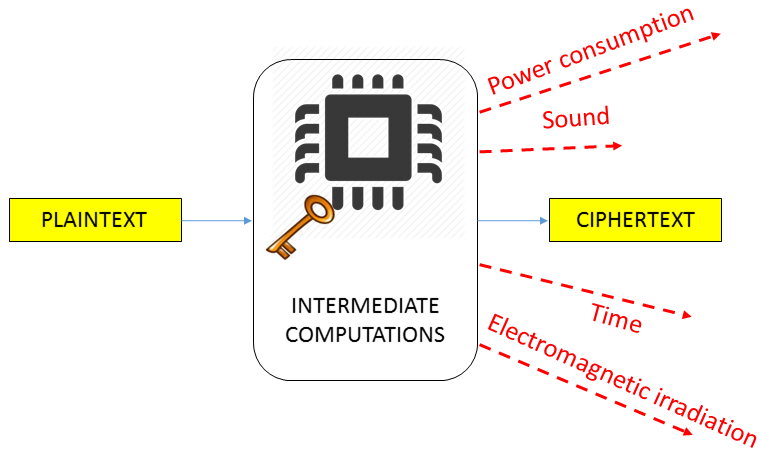
\includegraphics[width=0.5\textwidth]{Figures/channels}
	\caption{The different side channels encountered by an electronic device.
	Courtesy of Eleonora Cagli.}
	\label{fig:side_channels}
\end{wrapfigure}
Inside the electronic device, all the data related to the cryptographic primitive -- \ie{} the plaintexts, the secret key, the ciphertexts and all the intermediate computations -- are stored in the memory, loaded through the bus, and manipulated in the \gls{cpu} registers, under the physical form of electric signals.
All those elements are made of gates whose power consumption depends on the binary data they are supposed to store or to drive.
Therefore, depending on the processed data, an oscilloscope can notice slight changes in the measured power consumption, so an attacker can monitor this physical measurement to recover some information about the key, and thereby breaking the target device, as shown by Kocher~\cite{kocher_dpa_1999}.
A more detailed discussion about this dependency is proposed in \autoref{sec:non_profiled_attacks}.

Likewise, any change of value in the data passed through a given gate would result in a change of current in the gate, resulting in the emission of \glsfirst{em} radiations, which can be monitored thanks to an \gls{em} probe~\cite{gandolfi_electro_2001,quisquater_ema_2001}.

Other non-desired channels can be exploited by a malicious person: the intermediate computations processed by the electronic device can emit specific sounds allowing to distinguish secret values~\cite{genkin_rsa_2014}.
Moreover, if until a few years ago it was thought that only small devices, equipped with slow micro-processors and with small-sized architecture, such as smart cards, were vulnerable to this kind of side-channel attacks, the last cited recent work about acoustic emanations, together with other works exploiting electro-magnetic fluctuations, pointed out that much faster and bigger devices, \ie{} laptops and desktop computers, are vulnerable as well~\cite{genkin_get_2015,genkin_stealing_2015,genkin_ecdh_2016}.
Finally, the runtime of the implementation of a cryptographic primitive can also carry some sensitive information -- \ie{} depending on secret values, as emphasized by the seminal work of Kocher in 1996~\cite{kocher_timing_1996}.
This is particularly true when the implementation of the cryptographic primitive contains branches whose evaluation depends on sensitive values: if the different branches do not have the same runtime, it is therefore possible to guess which branch has been selected, which in turn provides information on the secret-related variable tested to branch.
Recently, in 2018, Kocher \etal{} proposed a timing attack based on modern \gls{cpu}'s architectures, involving low-level optimizations such as \emph{branch prediction} and \emph{speculative execution}~\cite{kocher_spectre_2018}.
Those optimization tricks concern nowadays most of the \glspl{cpu} such as \textsc{Intel}, \textsc{Amd}, or \textsc{Arm} processors, therefore making the vulnerability pervasive.
